\documentclass{article}
\usepackage[utf8]{inputenc}
\usepackage[english,ngerman]{babel}
%% ========================================================================
%%%% MISC usepackages
%% ========================================================================

%% Chemistry
\usepackage{chemfig,chemmacros}
\chemsetup{modules = all}
\chemsetup[redox]{explicit-sign = true}
\chemsetup[phases]{pos=sub}
%\chemsetup[reactions]{before-tag = {R}, tag-open = [, tag-close = ]}
  
%% Maths
\usepackage{amsmath,amssymb,amsthm,textcomp}

%% Physics
\usepackage{siunitx}

%% Graphics
\usepackage{graphicx}
\usepackage{tikz}
\usepackage{rotating}
%\usepackage{subfig}

%% Tables and Lists
\usepackage{enumerate}
\usepackage{multicol}
\usepackage{geometry}
\usepackage{tabu}
\usepackage{listings}
\usepackage{tabularx}

%% Structures and Style
\usepackage{caption}
\usepackage{subcaption}
\usepackage{booktabs}
\usepackage{colortbl}

\usepackage{xcolor}
\usepackage{xfrac}
\usepackage[export]{adjustbox}[2011/08/13]

\usepackage{booktabs}
\usepackage{float}

%% Citing and Settings
\usepackage[backend=biber,
style=numeric,
backref=true, 
natbib=true, %% offering natbib-compatible commands
hyperref=true, %% using hyperref-package references
sorting= none,
doi=true,
maxcitenames=10,
maxbibnames=100,
citestyle=numeric
]{biblatex}

\addbibresource{references.bib}

\usepackage[toc,automake]{glossaries}
\include{abbrevations}
\makeglossaries

\usepackage[colorlinks=true,linkcolor=blue]{hyperref}

%% Figure settings
\renewcommand{\figurename}{Abbildung}
\renewcommand{\tablename}{Tabelle}
\renewcommand{\listfigurename}{Abbildungsverzeichnis}
\renewcommand{\listtablename}{Tabellenverzeichnis}

%% ========================================================================
%%%% Document Information
%% ========================================================================

%% Title
\title{Dünnschicht- und Säulenchromatographie} % Title
\author{Autor: Florian \textsc{Kluibenschedl}} % Author name
\date{Bericht verfasst am: \today} % Date for the report

\begin{document}
  \renewtagform{reaction}[Rgl. ]{}{}
  
  \maketitle % Insert the title, author and date
  
  \begin{center}
    \begin{tabular}{r l}
      Versuchsdurchführung am: & 04. März 2019\\ % Date the experiment was performed
      Gruppe, Matrikelnummer: & 3, 11805747 \\
      Assistent: & Professor Smith % Instructor/supervisor
    \end{tabular}
  \end{center}


  \begin{abstract}
    
  \end{abstract}
  
  \section{Trennung von Aminosäuren - Dünnschichtchromatographie}
  
    \subsection{Theoretische Grundlagen}
  
      \subsubsection{Motivation} \label{sec:Motivation}
        
        Aminosäuren spielen eine grundlegende Rolle in vielen biochemischen Vorgängen. Werden sie über eine Peptidbindung miteinander verknüpft, bilden sie Polypeptide und in weiterer Folge Proteine. Um nun die oft sehr komplexe Funktionsweise der Proteine besser zu verstehen, ist es notwendig, ihren chemischen Aufbau zu kennen - also die Aminosäurensequenz. Die Möglichkeiten diese zu bestimmen reichen von ausgeklügelten spektroskopischen Methoden über spezifische Abbaureaktionen\footnote{z. B. Hydrolyse der Amidbindung} bis zu chromatographischen Methoden. 
        
        Die Dünnschichtchromatographie ist eine schnelle Methode \cite[S. 148]{TaschenatlasAnallytik}, ein Aminosäurengemisch ohne viel apparativen Aufwand aufzutrennen. Gründe für die Trennung sind Polaritätsunterschiede und verschiedene Dissoziationszustände\footnote{unter den Aminosäuren} bei gleichem \pH Wert\footnote{Aminosäuren haben typischerweise zwei unterschiedliche \pKa Werte (aufgrund der Carbonsäure- und der Aminogruppe), weswegen bei unterschiedlichen \pH Werten unterschiedliche Ionen zu erwarten sind - das Zwitterion liegt am isoelektrischem Punkt vor}. Durch Vergleich mit Referenzmessungen kann dann die genaue Zusammensetzung vom Aminosäurengemisch bestimmt werden.

      \subsubsection{Ziel des Experiments}
        
        Auf Basis der obigen Überlegungen ist das Ziel, die Zusammensetzung einer Aminosäurenmischung\footnote{mindestens zwei Aminosäuren sind enthalten} zu bestimmen. Die Auswahl ist dabei beschränkt auf L-Serin, L-Leucin, L-Prolin, L-Arginin und L-Histidin.
    
    \subsection{Experimenteller Teil}
  
      \subsubsection{Verwendete Materialien}
              
        \begin{table}[H]
          \centering
          \caption[Materialienliste Dünnschichtchromatographie, Quelle: Autor]{Auflistung der verwendeten Geräte und Chemikalien}
          \label{tab:Materialien}
        
          \begin{tabular}{@{}ll|p{4.5cm}l@{}}
            \toprule
              Geräte & Hersteller & Chemikalie & Bezogen von \\ \midrule
              DC-Platte &  & neutrales Laufmittel - \SI[mode=text]{30}{\milli\litre} \ch{CH3CN}, \SI[mode=text]{20}{\milli\litre} \SI[mode=text]{0.1}{M} \ch{NH4Ac}, \SI[mode=text]{25}{\milli\litre} Ethanol & Vorrat \\
              \SI[mode=text,separate-uncertainty=true]{250}{\milli\litre} Becherglas &  & saures Laufmittel - \SI[mode=text]{30}{\milli\litre} n-Butanol, \SI[mode=text]{10}{\milli\litre} deion. \ch{H2O}, \SI[mode=text]{10}{\milli\litre} konz. Eisessig & Vorrat \\
              Uhrglas &  & verdünnte L-Serin Lösung &  \\
              Föhn &  & verdünnte L-Leucin Lösung &  \\
              Glaskapillaren &  & verdünnte L-Prolin Lösung &  \\
              Trockenschrank &  & verdünnte L-Arginin Lösung &  \\
              \SI[mode=text]{14}{\centi\meter} Geodreieck und Bleistift &  & verdünnte L-Histidin Lösung &  \\
                &  & \SI[mode=text]{0.1}{\percent} (w/w) Ninhydrin Lösung in Ethanol &  \\ \bottomrule
          \end{tabular}
        \end{table}
        
        Anmerkung zur Handhabung von Ninhydrin\footnote{H und P Sätze: H - 302, 315, 319, 335; P - 261, 305, 351, 338}: Haut, Atemwege und Augen werden gereizt - bei Kontakt mit Wasser spülen
        
      \subsubsection{Versuchsdurchführung} \label{sec:Versuch}
        
        \begin{figure}[H]
          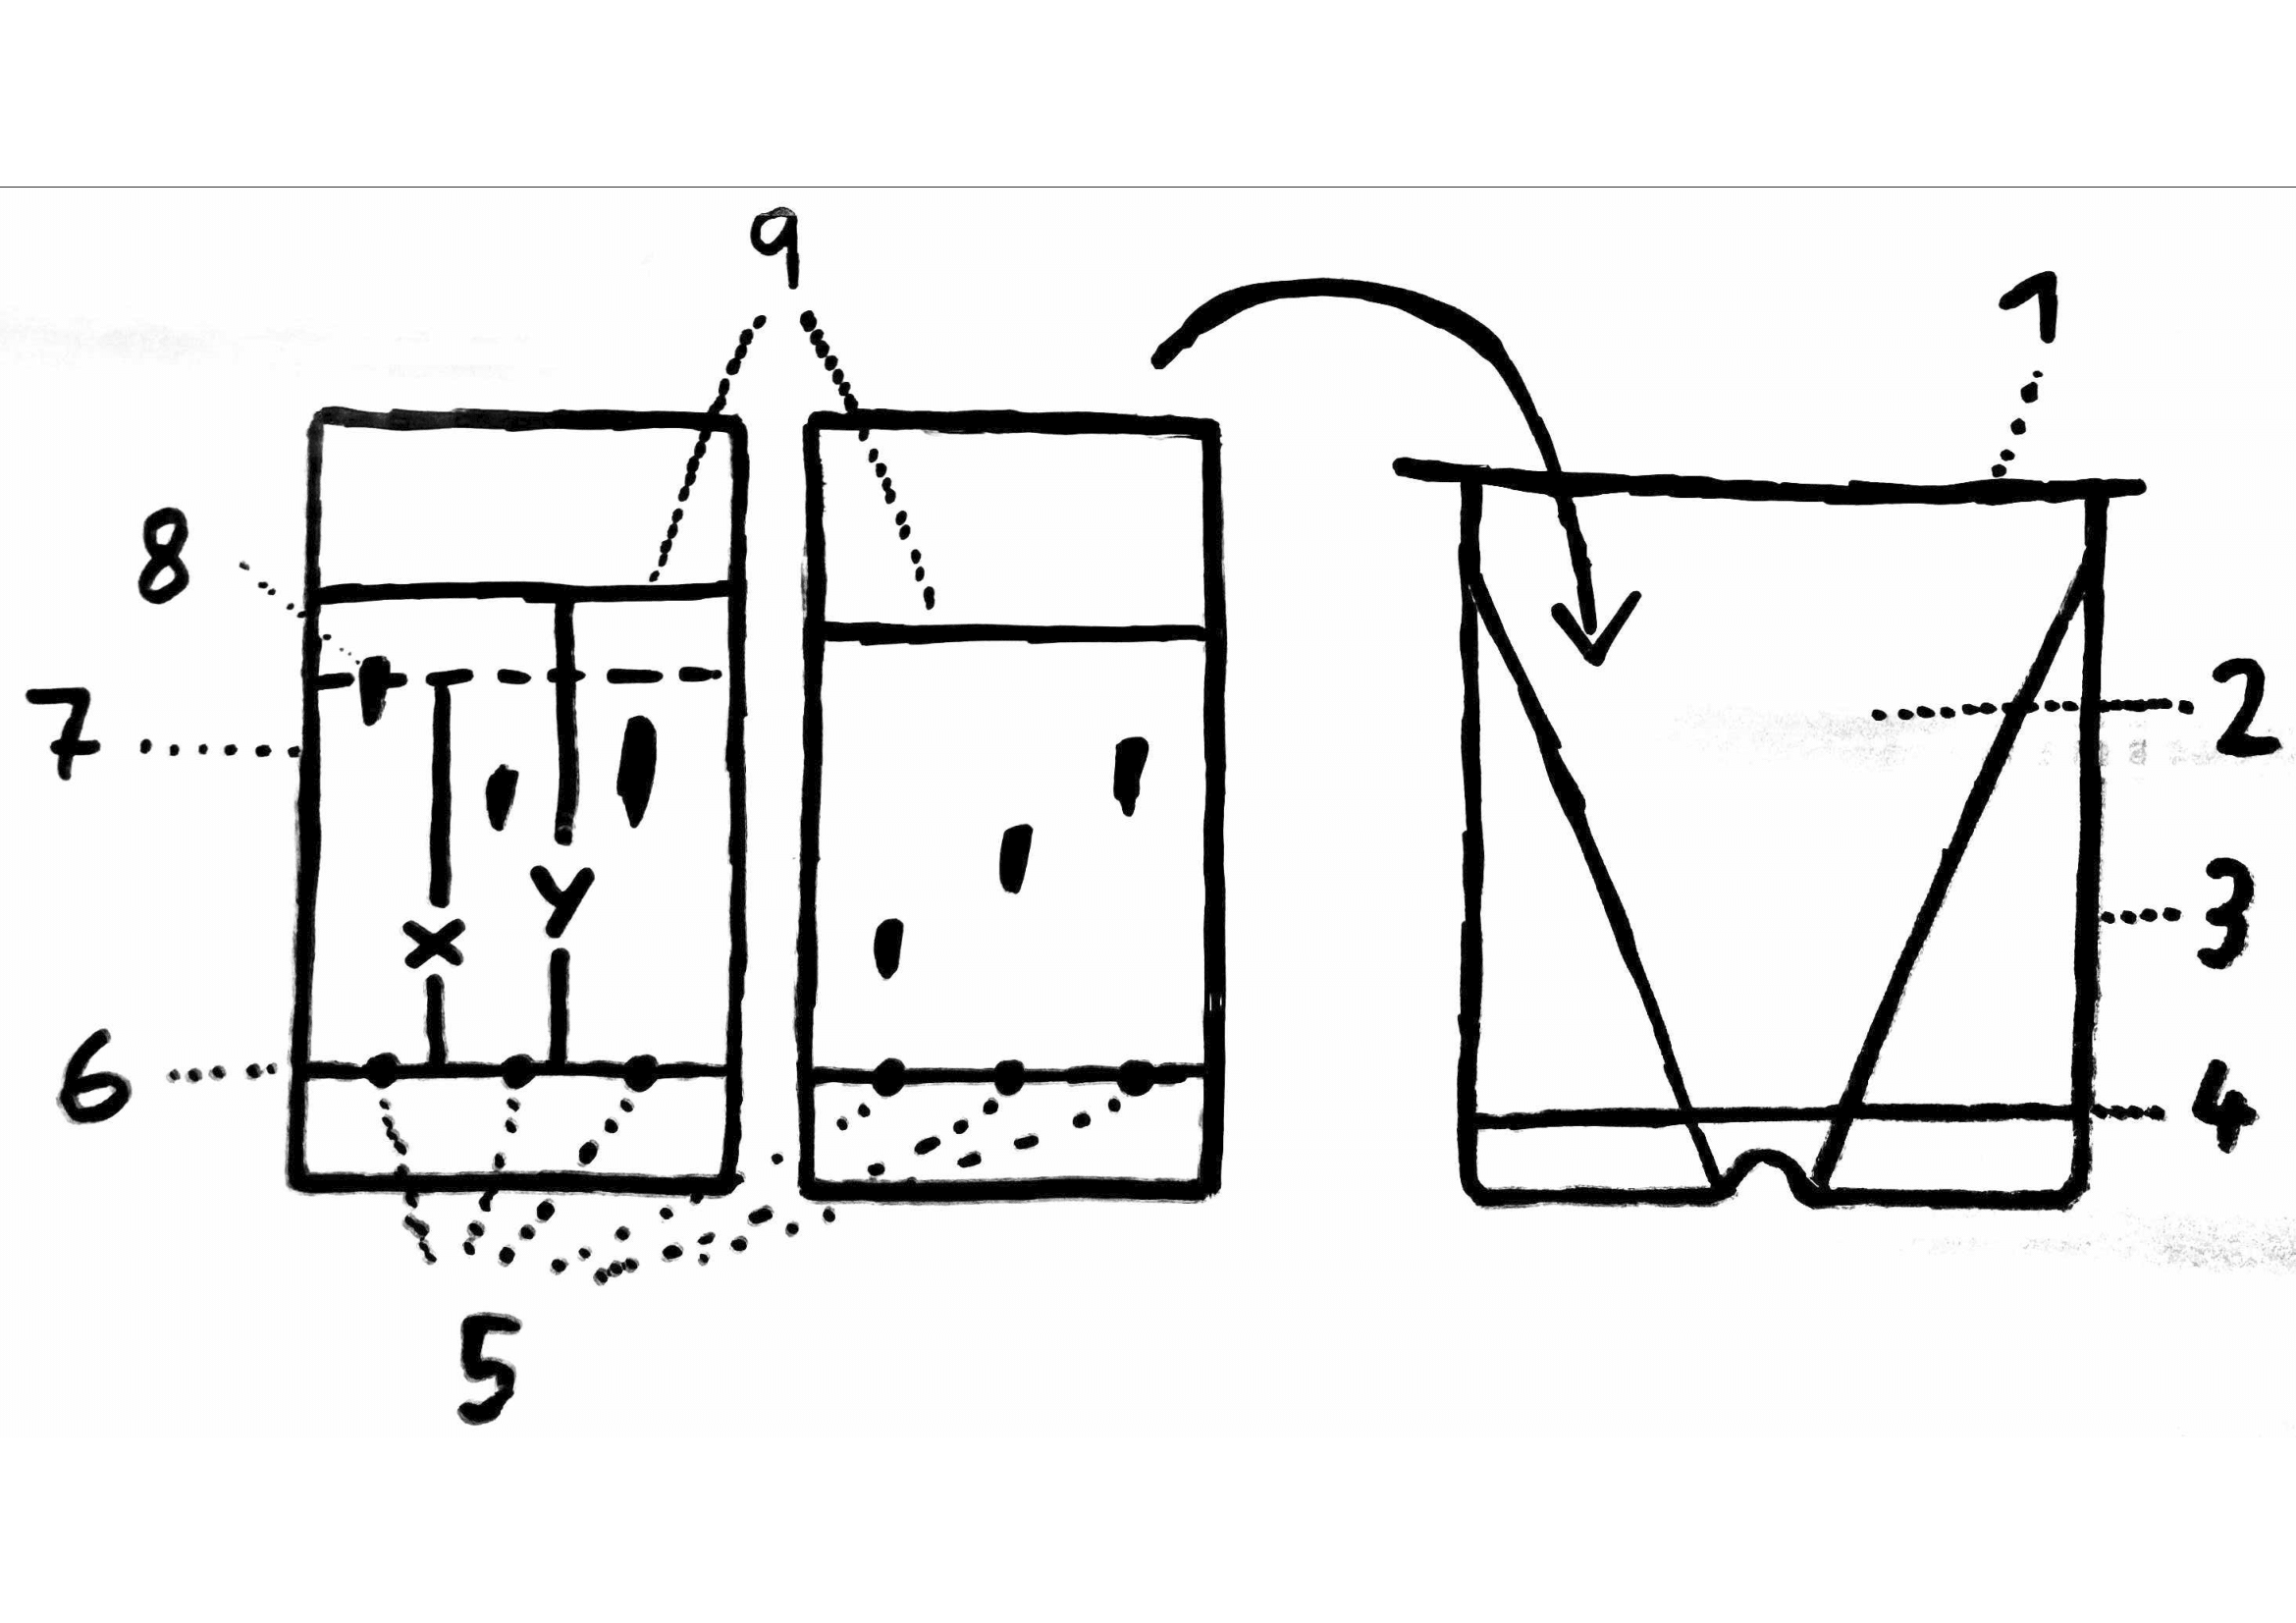
\includegraphics[scale=0.08, center]{Graphiken/Versuchsanordnungen/VersuchsanordnungDC.png} 
          \caption[schematische Versuchsanordnung Dünnschichtchromatographie, Quelle: Autor]{schematische Versuchsanordnung: (1) Uhrglas, (2) mit Lösungsmitteldämpfen gesättigter Gasraum, (3) DC-Kammer - \SI[mode=text,separate-uncertainty=true]{250}{\milli\litre} Becherglas, (4) Laufmittelstand - ca. \SI[mode=text]{0.5}{\centi\meter} über dem Boden des Becherglases, (5) Probespots, (6) mit Bleistift markierte Startlinie, (7) DC-Platte, (8) Probespots nach erfolgter Trennung, (9) Laufmittelfronten - nach Entnahme der DC-Platte mit Bleistift markiert}
          \label{fig:Versuchsanordnung}
        \end{figure}
    
        Zu Beginn wurde die DC-Kammer mit dem jeweiligem Laufmittel\footnote{es wurden zwei Laufmittel verwendet, die Zusammensetzung ist in Tabelle \ref{tab:Materialien} beschrieben} gefüllt, wie in Abbildung \ref{fig:Versuchsanordnung} beschrieben. Das Becherglas wurde mit dem Uhrglas bedeckt, um die DC-Kammer mit dem Lösungsmitteldampf zu sättigen. 
        
        Auf zwei DC-Platten wurde in einer Höhe von \SI[mode=text]{1}{\centi\meter} je eine Startlinie eingezeichnet. Auf dieser wurden dann in regelmäßigem Abstand Probespots der gegebenen fünf Aminosäuren und der zu untersuchenden Probe aufgetragen\footnote{mithilfe einer Kapillare, die vor jeder neuen Probenaufnahme gereinigt wurde}. Es wurde darauf geachtet, große Probespots zu vermeiden (max. Durchmesser von \SI[mode=text]{2}{\milli\meter}). Nach dem Trocknen der Spots wurden die DC-Platten in die wie oben beschrieben präparierte DC-Kammer gestellt (wie in Abbildung \ref{fig:Versuchsanordnung} zu sehen) und mit dem Uhrglas abgedeckt. Nachdem die Laufmittelfront ca. 2/3 der Platte erreichte, wurde sie aus der DC-Kammer entnommen und die Laufmittelfront mit einem Bleistift markiert. Nach dem Trocknen wurde die DC-Platte im Abzug mit einer Ninhydrin Lösung besprüht und kurz geföhnt. Anschließend wurde sie im Trockenschrank bei \SI[mode=text]{110}{\degreeCelsius} entwickelt.
    
      \subsubsection{Auswertung}
    
        Aufgrund der in \ref{sec:Motivation} genannten, unterschiedlichen Eigenschaften der untersuchten Proben, halten sich die einzelnen Substanzen verschieden lange in der stationären\footnote{Kieselgel der DC-Platte} bzw. der mobilen \footnote{Laufmittel} Phase auf. Damit legen sie unterschiedliche Strecken auf der DC-Platte zurück, die für eine  Substanz charakteristisch, also reproduzierbar sind\footnote{natürlich bei gleicher Laufmittelzusammensetzung}. Aus der zurückgelegten Strecke der Substanz ($= x$) und der zurückgelegten Strecke des Laufmittels ($= y$) errechnet sich der Retentionsfaktor wie in \eqref{eq:Rf} dargestellt.
    
        \begin{equation}
          R_{f} = \frac{x}{y} \label{eq:Rf}
        \end{equation}
      
      \subsubsection{Messergebnisse}
    
        In Tabelle \ref{tab:Messdaten} sind alle Messwerte, die im Rahmen der Versuchsdurchführung wie in \ref{sec:Versuch} beschrieben, gemessen wurden. Die Werte von $y_{sauer}, y_{neutral}$ separat: $y_{sauer} = $ \SI[mode=text]{}{\centi\meter}, $y_{neutral} = $ \SI[mode=text]{}{\centi\meter}.
      
        \begin{table}[H]
          \centering
          \caption[Messdaten, Quelle: Autor]{Messdaten}
          \label{tab:Messdaten}
            \begin{tabular}{@{}l|ll|ll@{}}
              \toprule
               Substanz & $x_{sauer}$ in \si{\centi\meter} & $R_{f,sauer}$ & $x_{neutral}$ in \si{\centi\meter} & $R_{f,neutral}$ \\ \midrule
               L-Serin &  & & \\
               L-Leucin &  &  &  \\
               L-Prolin &  &  &  \\
               L-Arginin &  &  &  \\
               L-Histidin &  &  &  \\ \midrule
               Probe &  &  &  \\
                     &  &  &  \\
                     &  &  &  \\ \bottomrule
            \end{tabular}
         \end{table}      
      
    \subsection{Ergebnisse und Diskussion}
  
  \section{Trennung von Pflanzenfarbstoffen - Säulenchromatographie}
  
    \subsection{Theoretische Grundlagen}
    
      \subsubsection{Motivation} \label{sec:Motivationzwei}
      
        Säulenchromatographie ist analog zur Dünnschichtchromatographie eine Methode zum Trennen einer Substanzmischung. Die stationäre Phase ist in einer Säule gepackt. Die Probe wird am Anfang der Säule aufgegeben und anschließend wird kontinuierlich Eluent (= mobile Phase) hinzugeben. Die Retentionszeit gibt an, wie lang eine Substanz braucht, um durch die Säule zu wandern. Aufgrund der unterschiedlich starken Wechselwirkungen der einzelnen Substanzen mit der stationären Phase, werden die Substanzen getrennt. Der apparative aufwand ist im Vergleich zur Dünnschichtchromatographie etwas größer, hält sich jedoch in Grenzen \cite[S. 154]{TaschenatlasAnallytik}.\\
        
        Die beiden Biomoleküle Chlorophyll und Carotin nehmen eine bedeutende Rolle im Leben ein. Chlorophyll ist für die grüne Blattfarbe verantwortlich und überlagert zunächst das Carotin. Dieses kommt jedoch zum Vorschein, wenn im Herbst das Chlorophyll systematisch abgebaut wird \cite{DegradationChlorophyll}. 
      
      \subsubsection{Ziel des Experiments}
      
        Um die Eigenschaften der beiden in \ref{sec:Motivationzwei} genannten Moleküle genauer zu bestimmen, müssen diese zuerst voneinander getrennt werden. Das Ziel des Experiments ist somit, mithilfe von Säulenchromatographie eine entsprechende Trennung durchzuführen. Als Probenmaterial wurden Spinatblätter verwendet.
    
    \subsection{Experimenteller Teil}
    
      \subsubsection{Verwendete Materialien}
        
        \begin{table}[H]
          \centering
          \caption[Materialienliste Säulenchromatographie, Quelle: Autor]{Auflistung der verwendeten Geräte und Chemikalien}
          \label{tab:Materialienzwei}
        
          \begin{tabular}{@{}ll|ll@{}}
            \toprule
              Geräte & Hersteller & Chemikalie & Bezogen von \\ \midrule
              Pasteurpipette mit Saugaufatz &  & Spinatblätter (\textit{lat. Spinacia oleracea}) & Vorrat \\
              \SI[mode=text,separate-uncertainty=true]{10.0(1)}{\milli\litre} Messzylinder &  & Petrolether & Vorrat \\
              Reagenzgläser &  & Ethanol &  \\
              \SI[mode=text,separate-uncertainty=true]{50}{\milli\litre} Becherglas &  & Aceton &  \\
               &  & \ch{Al2O3} &  \\
               &  & Glaswolle &  \\
               &  & Sand &  \\ \bottomrule
          \end{tabular}
        \end{table}
        
      \subsubsection{Versuchsdurchführung} \label{sec:Versuchsdurchzwei}
        
        \begin{figure}[H]
          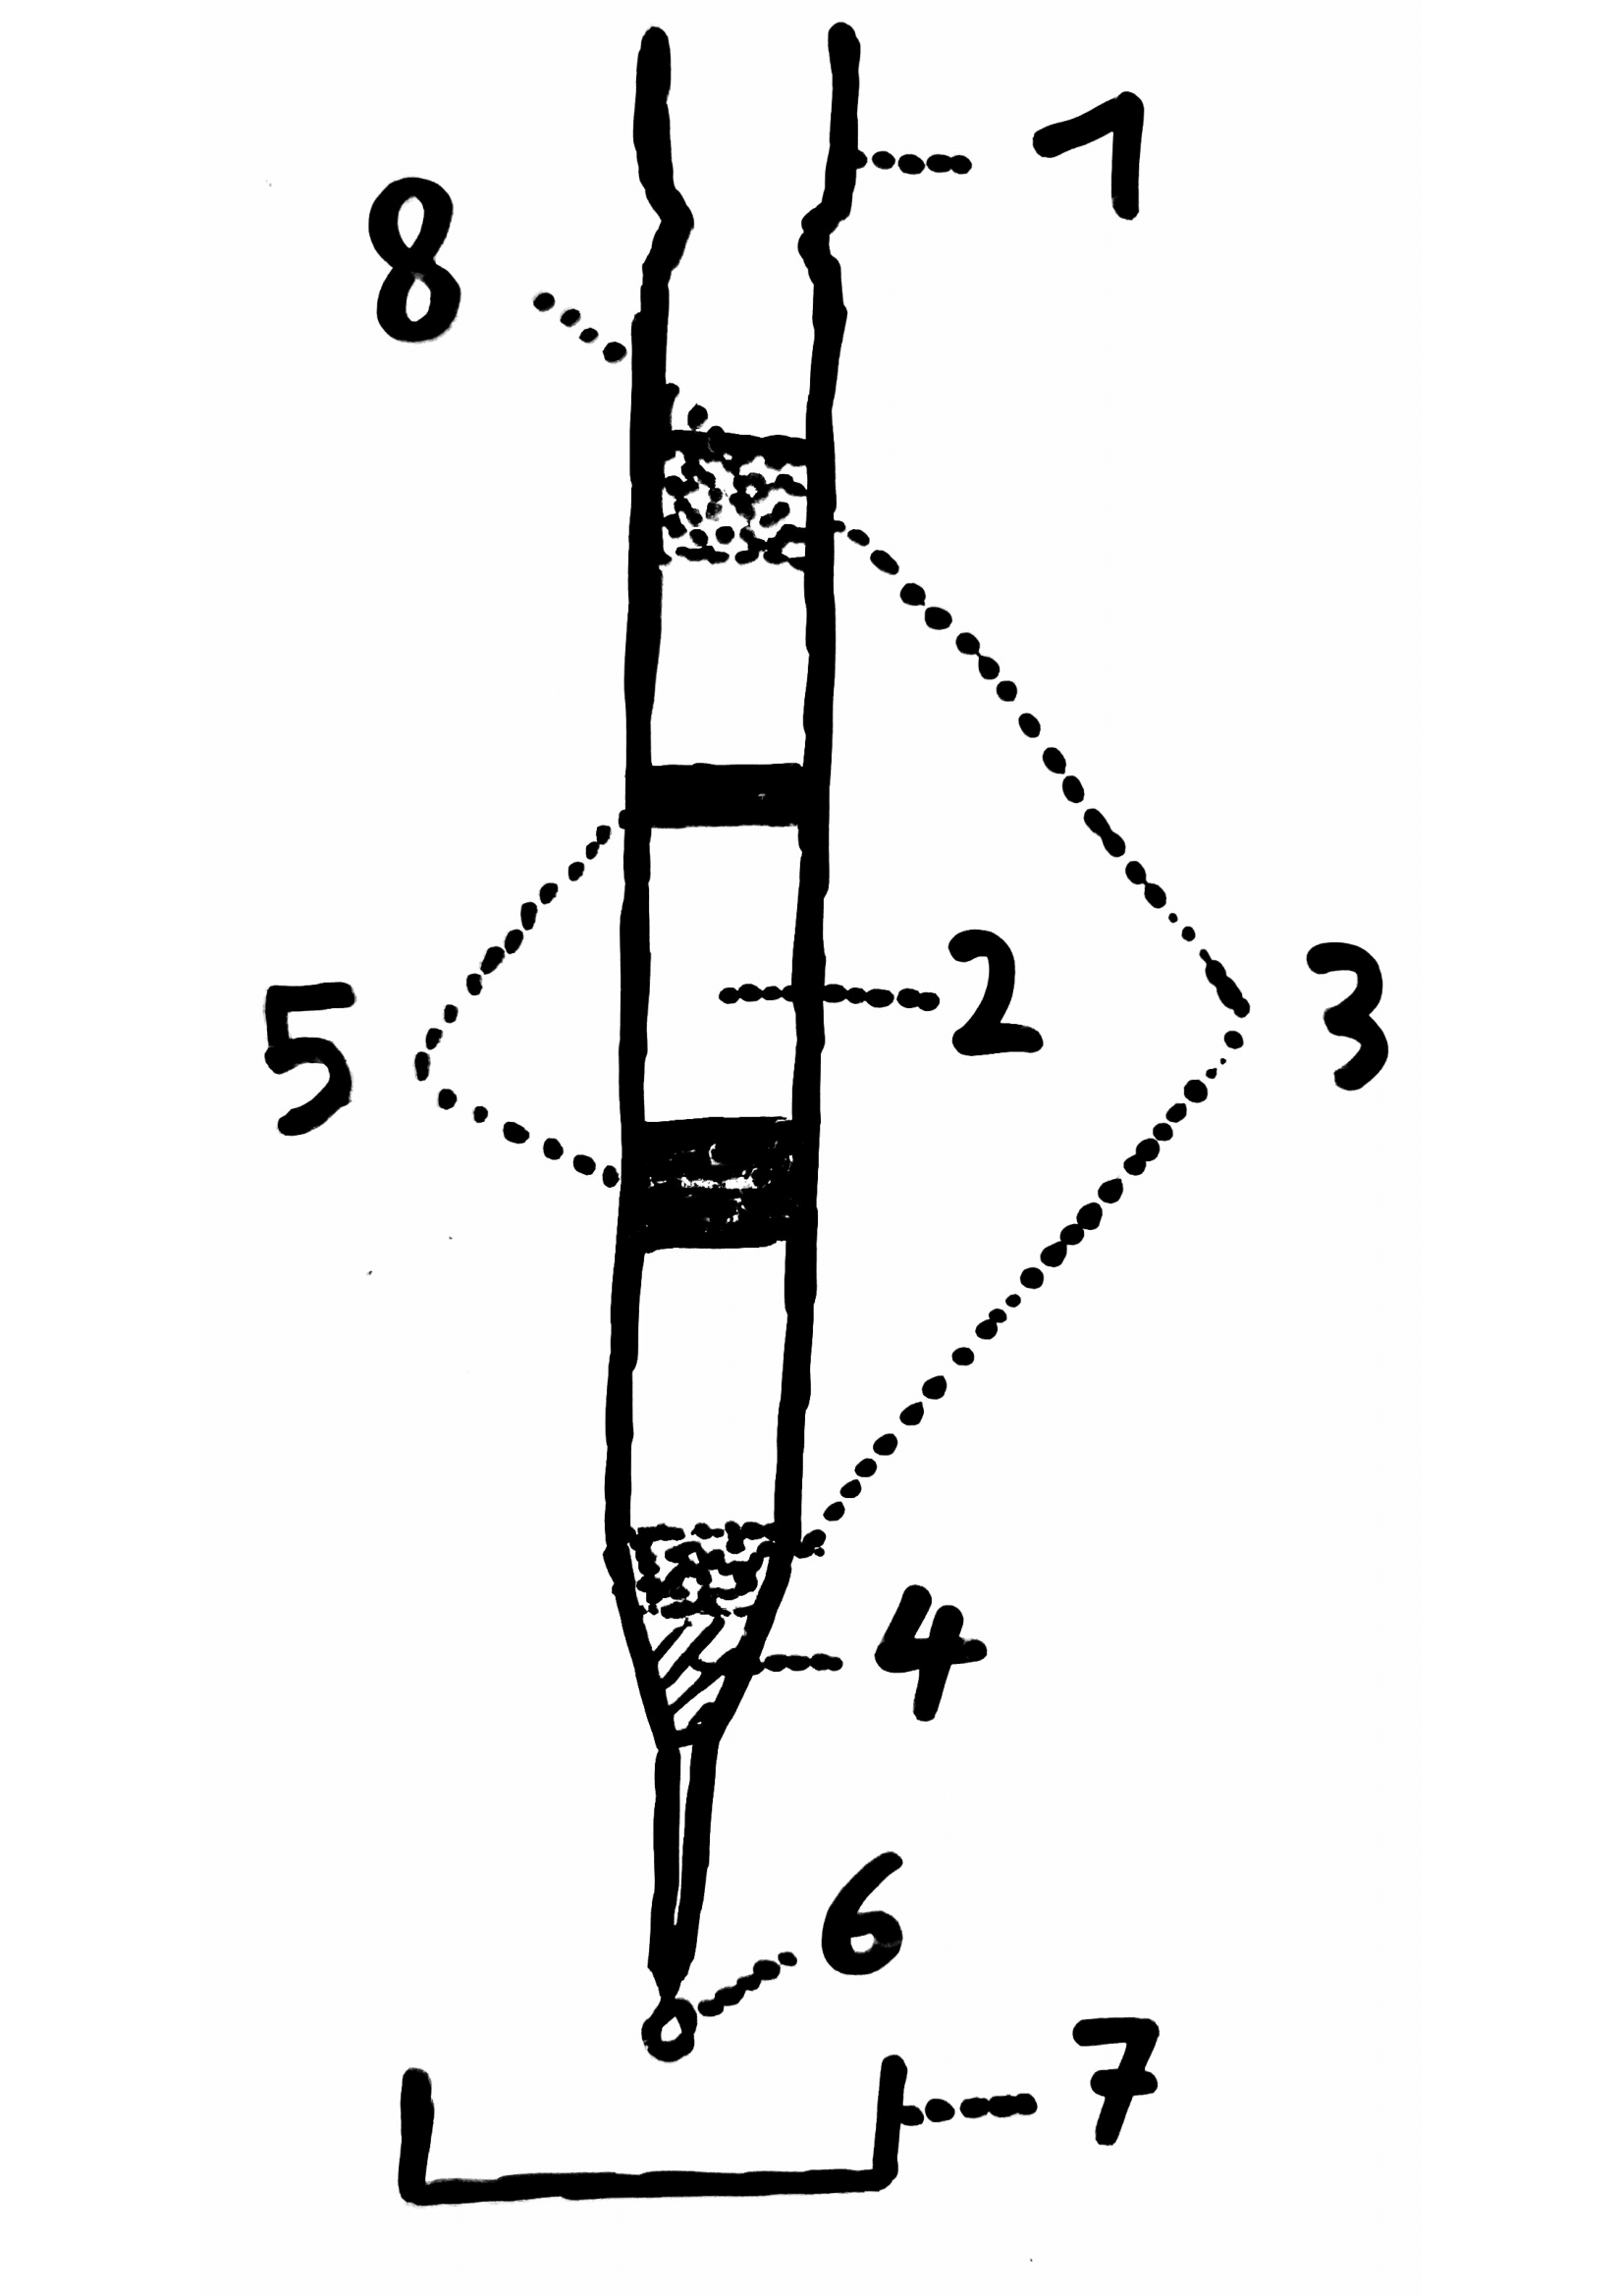
\includegraphics[scale=0.08, center]{Graphiken/Versuchsanordnungen/VersuchsanordnungSC.png} 
          \caption[schematische Versuchsanordnung Säulenchromatographie, Quelle: Autor]{schematische Versuchsanordnung: (1) Pasteurpipette - Säule - und Öffnung für Eluentenzufuhr, (2) ca. \ch{Al2O3}-Schicht, (3) Sand, (4) Glasswolle, (5) Banden der getrennten Substanzen, (6) Ort der Elution der Subtanz, (7) Auffangvorrichtung, (8) Aufgabe der Probe}
          \label{fig:Versuchsanordnungzwei}
        \end{figure}
        
        Im ersten Schritt wurde eine Analysenlösung vorbereitet. Dazu wurde ein Spinatblatt im \SI[mode=text,separate-uncertainty=true]{50}{\milli\litre} Becherglas zerkleinert und mit ca. \SI[mode=text]{5}{\milli\litre} \ch{EtOH} gewaschen. Die \ch{EtOH}-Fraktion wurde abdekantiert und verworfen. Nun wurden \SI[mode=text]{5}{\milli\litre} Petrolether hinzugegeben und das Blattextrakt für ca. \SI[mode=text]{5}{\minute} lang durch Schütteln extrahiert. Es wurde wieder abdekantiert, wobei die Petrolether-Fraktion nicht verworfen und nicht zur Trennung eingesetzt wurde. 
        
        Nun wurden die Elutionslösungen\footnote{=mobilen Phase} vorbereitet. Elutionslösung 1 war eine Mischung von \SI[mode=text]{0.7}{\milli\litre} Aceton mit \SI[mode=text]{9.3}{\milli\litre} Petrolether. Elutionslösung 2 war reines Aceton. Beide Lösungen wurden griffbereit aufbewahrt.
        
        Die Trennsäule wurde wie in \ref{fig:Versuchsanordnungzwei} skizziert vorbereitet. Als Säule diente eine Pasteurpipette, die man mit einem Stativ befestigte. Zuerst wurde die Pipette mit Glaswolle befüllt, die mithilfe eines Drahtes schön kompakt zusammengedrückt wurde\footnote{desto kompakter, desto höher ist die Trennleistung aufgrund der größeren Anzahl an Wechselwirkungen}. Danach wurde diese mit einer ca. \SI[mode=text]{0.3}{\centi\meter} hohen Sandschicht überdeckt. In einem Reagenzglas wurde eine ca. \SI[mode=text]{1}{\centi\meter} dicke \ch{Al2O3}-Schicht mit \SI[mode=text]{7}{\centi\meter} Petrolether überdeckt. Durch Aufschlemmen des \ch{Al2O3} mit einer Pasteurpipette  erhielt man eine Suspension, die in die Säule überführt wurde, wobei darauf geachtet wurde, die Entstehung von Luftblasen in der Säule zu vermeiden. Ein Trockenlaufen der Säule wurde in allen folgenden Schritten durch konstante Zufuhr an Elutionslösung verhindert\footnote{beim Befüllen nach dem Trockenlaufen kann es zum Einschluss von Luft in der Säule kommen, was die Trennleistung reduziert}. Diese Schicht wurde mit einer ca. \SI[mode=text]{0.3}{\centi\meter} hohen Sandschicht überdeckt. 
        
        Nun konnte mit der Trennung gestartet werden. Dazu wurde die im ersten Schritt vorbereitete Analysenlösung auf die oberste Sandschicht gelegt\footnote{der Petrolether hat gerade die oberste Sandschicht durchquert} und gewartet, bis sie zur Gänze in die Sandschicht eingedrugen war\footnote{Vorgang auch als Beladen der Säule bezeichnet}. Elutionslösung 1 wurde hinzugegeben. Das Carotin löste sich in dieser besser wie das Chlorophyll und eine gelbe Bande wanderte die Säule hinunter. Am Säulenende angelangt, wurde die Fraktion in einem Reagenzglas aufgefangen, wie in \ref{fig:Versuchsanordnungzwei} gezeigt\footnote{Eluent 1}. Das Chlorophyll wurde durch einen Wechsel der Elutionslösung erhalten. Elutionslösung 2 wurde dazu verwendet. Analog zum Carotin wurde das Chlorophyll am Säulenende aufgefangen\footnote{natürlich in einem anderen Reagenzglas - Eluent 2}.
        
    \subsection{Ergebnisse und Diskussion}
    
      Nach dem Trennvorgang wurden zwei Lösungen erhalten - Eluent 1 mit Carotin und Eluent 2 mit Chlorophyll. Durch die unterschiedliche Farbe können sie eindeutig voneinander unterschieden werden, weswegen die Trennung als erfolgreich anzusehen ist.
      
  \pagebreak
  
  \listofreactions
  \printbibliography[title=Literaturverzeichnis]
  \listoffigures
  \listoftables
  
\end{document}
